\documentclass[aspectratio=43]{beamer}
\usetheme{default}

\usepackage{pgffor}
\usepackage{hyperref}
\usepackage{tikz}

\begin{document}

\title{Lazy List Sets}
\subtitle{VU Advanced Multiprocessor Programming}
\author{Thomas Weber}
\institute[TU]{Vienna University of Technology}
\date{\today}

\begin{frame}[plain] 
  \titlepage
\end{frame}

\begin{frame}{Lazy Set data-structure}
  \begin{itemize}
  \item{Set stored as a sorted list}
  \item{Fine-grained locking in \texttt{add()} and \texttt{remove()}}
  \item{Lock-free \texttt{contains()}}
  \end{itemize}
  
  \begin{itemize}
  \item{\textbf{BUT}: $O(n)$ complexity (vs.\ $O({log} n)$ of \texttt{std::set})}
  \end{itemize}

\end{frame}

\begin{frame}{List-based sets}
  \begin{itemize}
  \item{Also implemented other list-based sets from Herlihy\&Shavit}
  \item{Made sense since they build upon one another}
  \end{itemize}

  \begin{itemize}
  \item{\texttt{CoarseListSet}}
    \begin{itemize}
    \item{single global lock}
    \end{itemize}
  \item{\texttt{FineListSet}}
    \begin{itemize}
    \item{per-node locking as list is iterated}
    \end{itemize}
  \item{\texttt{OptimisticListSet}}
    \begin{itemize}
    \item{don't lock during iteration, but lock and check found nodes}
    \item{checking done by reiterating from beginning}
    \end{itemize}
  \item{\texttt{LazyListSet}}
    \begin{itemize}
    \item{use flags instead of reiteration to check validity}
    \item{same flag can also be used to avoid locking for \texttt{contains()}}
    \end{itemize}
  \end{itemize}

  % \begin{itemize}
  % \item{Also testing \texttt{GlobalLockSet}}
  %   \begin{itemize}
  %   \item{globally locked \texttt{std::set}}
  %   \end{itemize}
  % \end{itemize}
\end{frame}

\begin{frame}{Stress testing \texttt{add()}}
  \begin{figure}
    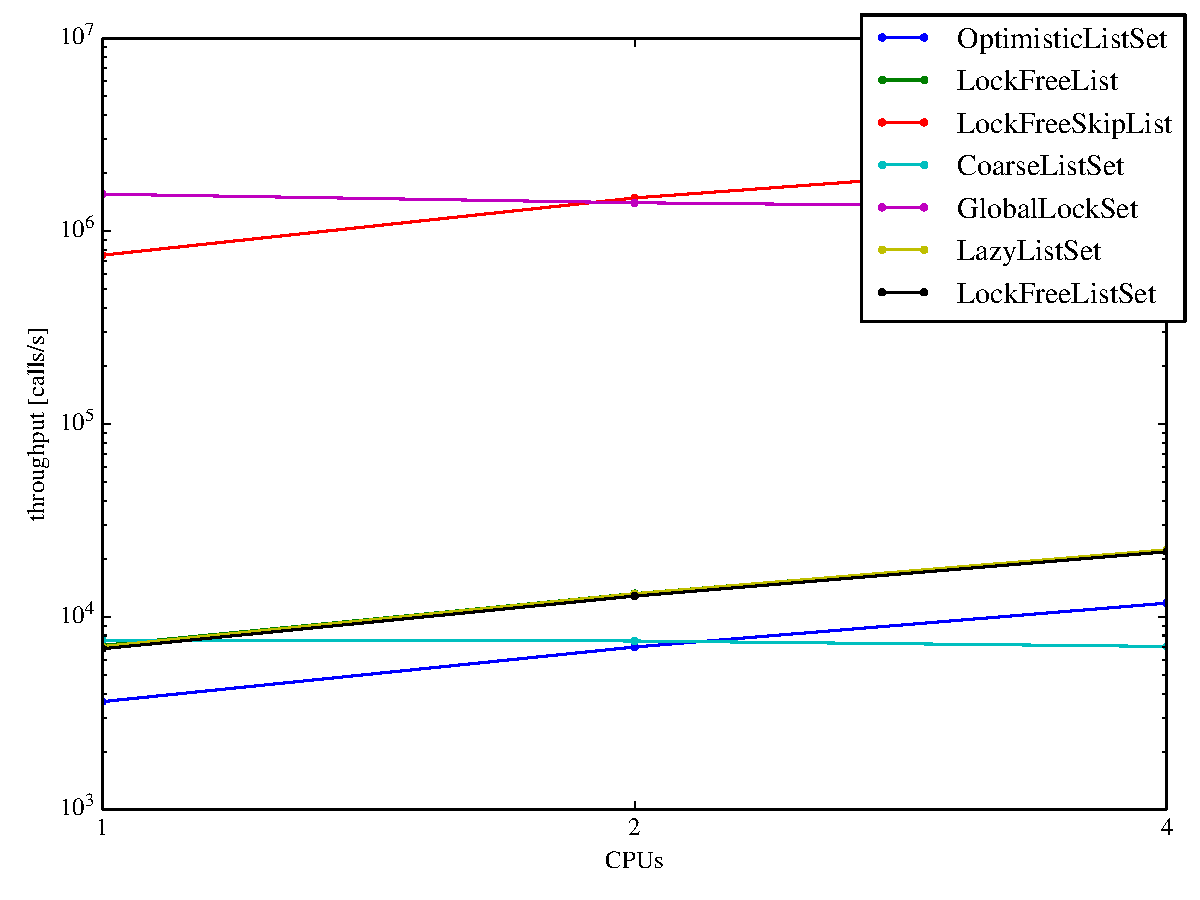
\includegraphics[width=\textwidth]{add}
  \end{figure}  
\end{frame}

\begin{frame}{Stress testing \texttt{remove()}}
  \begin{figure}
    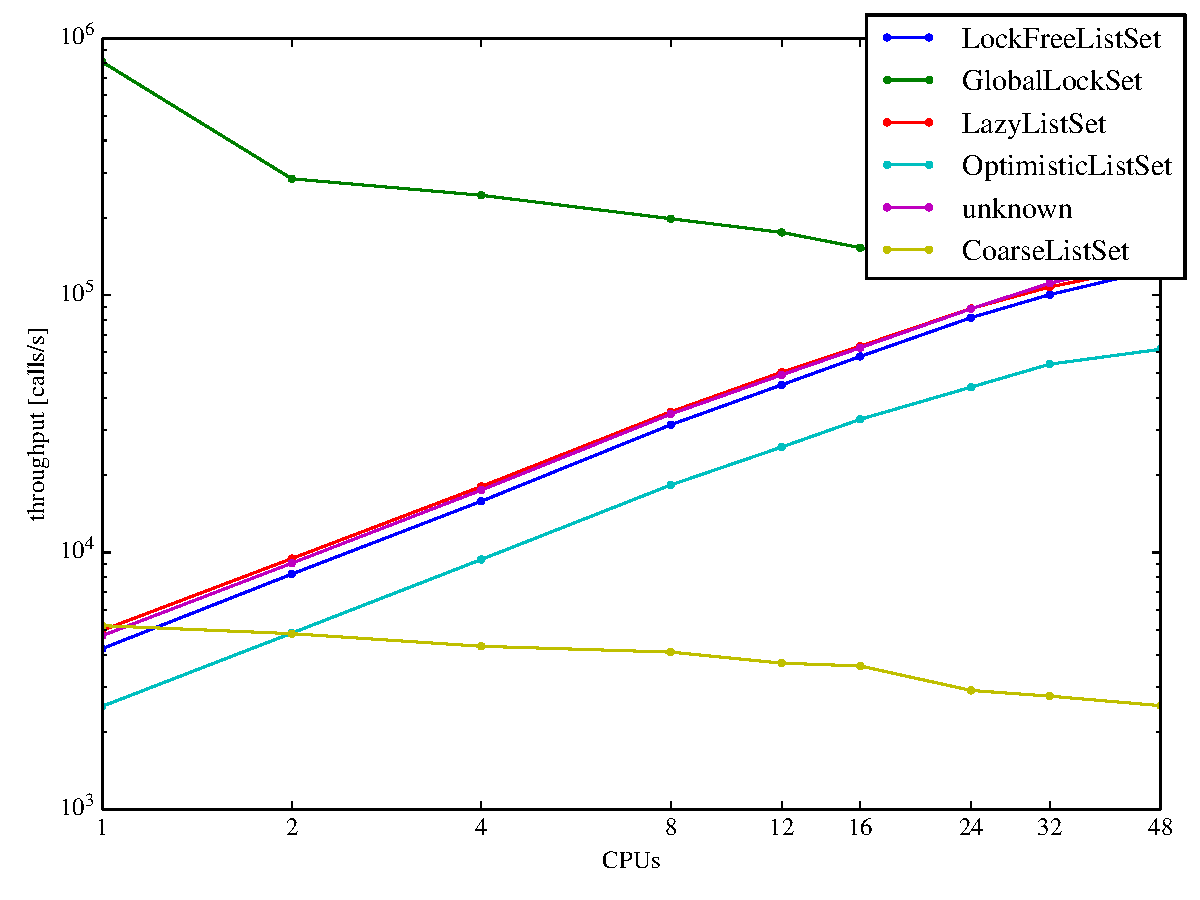
\includegraphics[width=\textwidth]{remove}
  \end{figure}  
\end{frame}

\begin{frame}{Stress testing \texttt{contains()}}
  \begin{figure}
    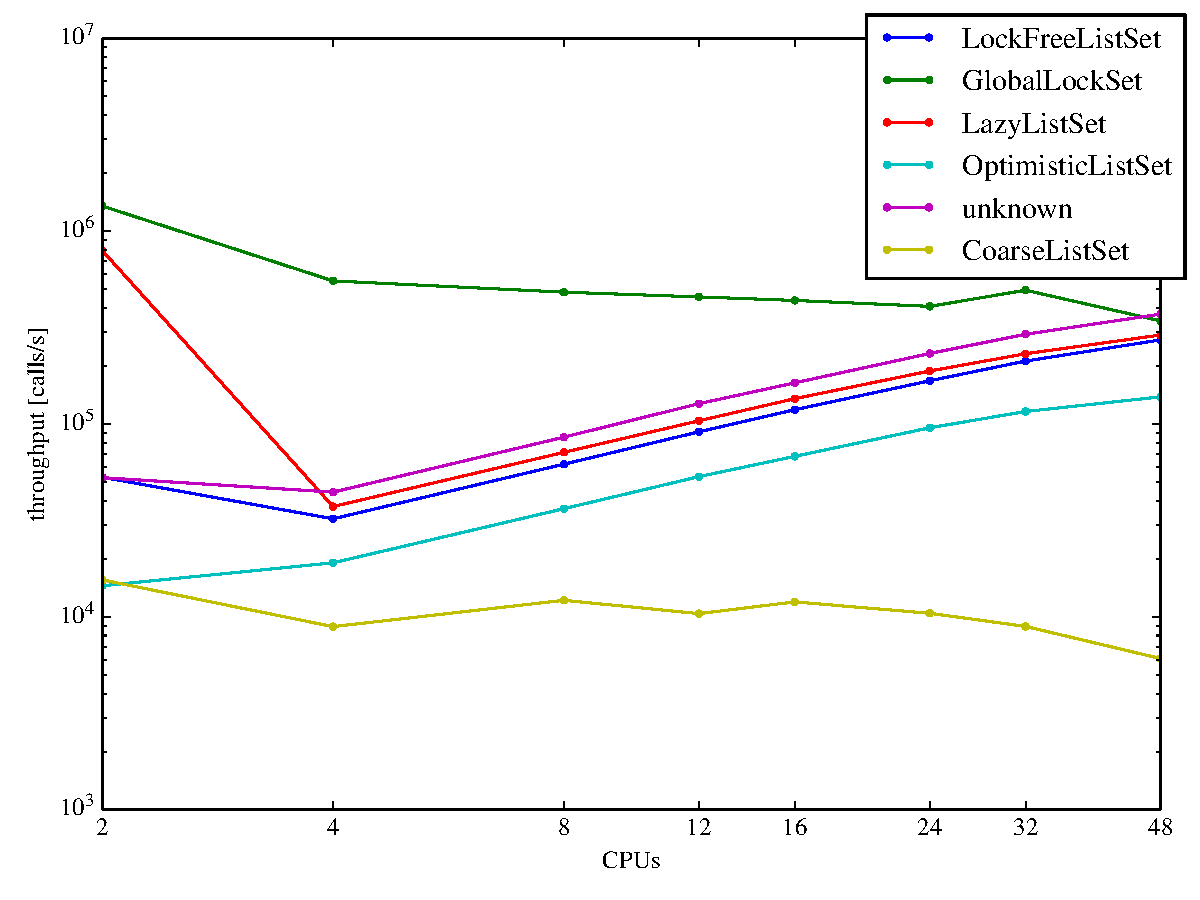
\includegraphics[width=\textwidth]{contains}
  \end{figure}  
\end{frame}



\end{document}
